% -*-Latex-*-
\title{How Drift Affects Heterozygosity}
\author{Alan R. Rogers}
\date{\today}
\frame{\titlepage}

\begin{frame}
We begin with data from an experiment, described by Peter Buri in
1956.  (Gene frequency in small populations of mutant
\emph{Drosophila}, Evolution, 10:367--402)
\end{frame}

\begin{frame}
\begin{columns}
\column{0.6\textwidth}
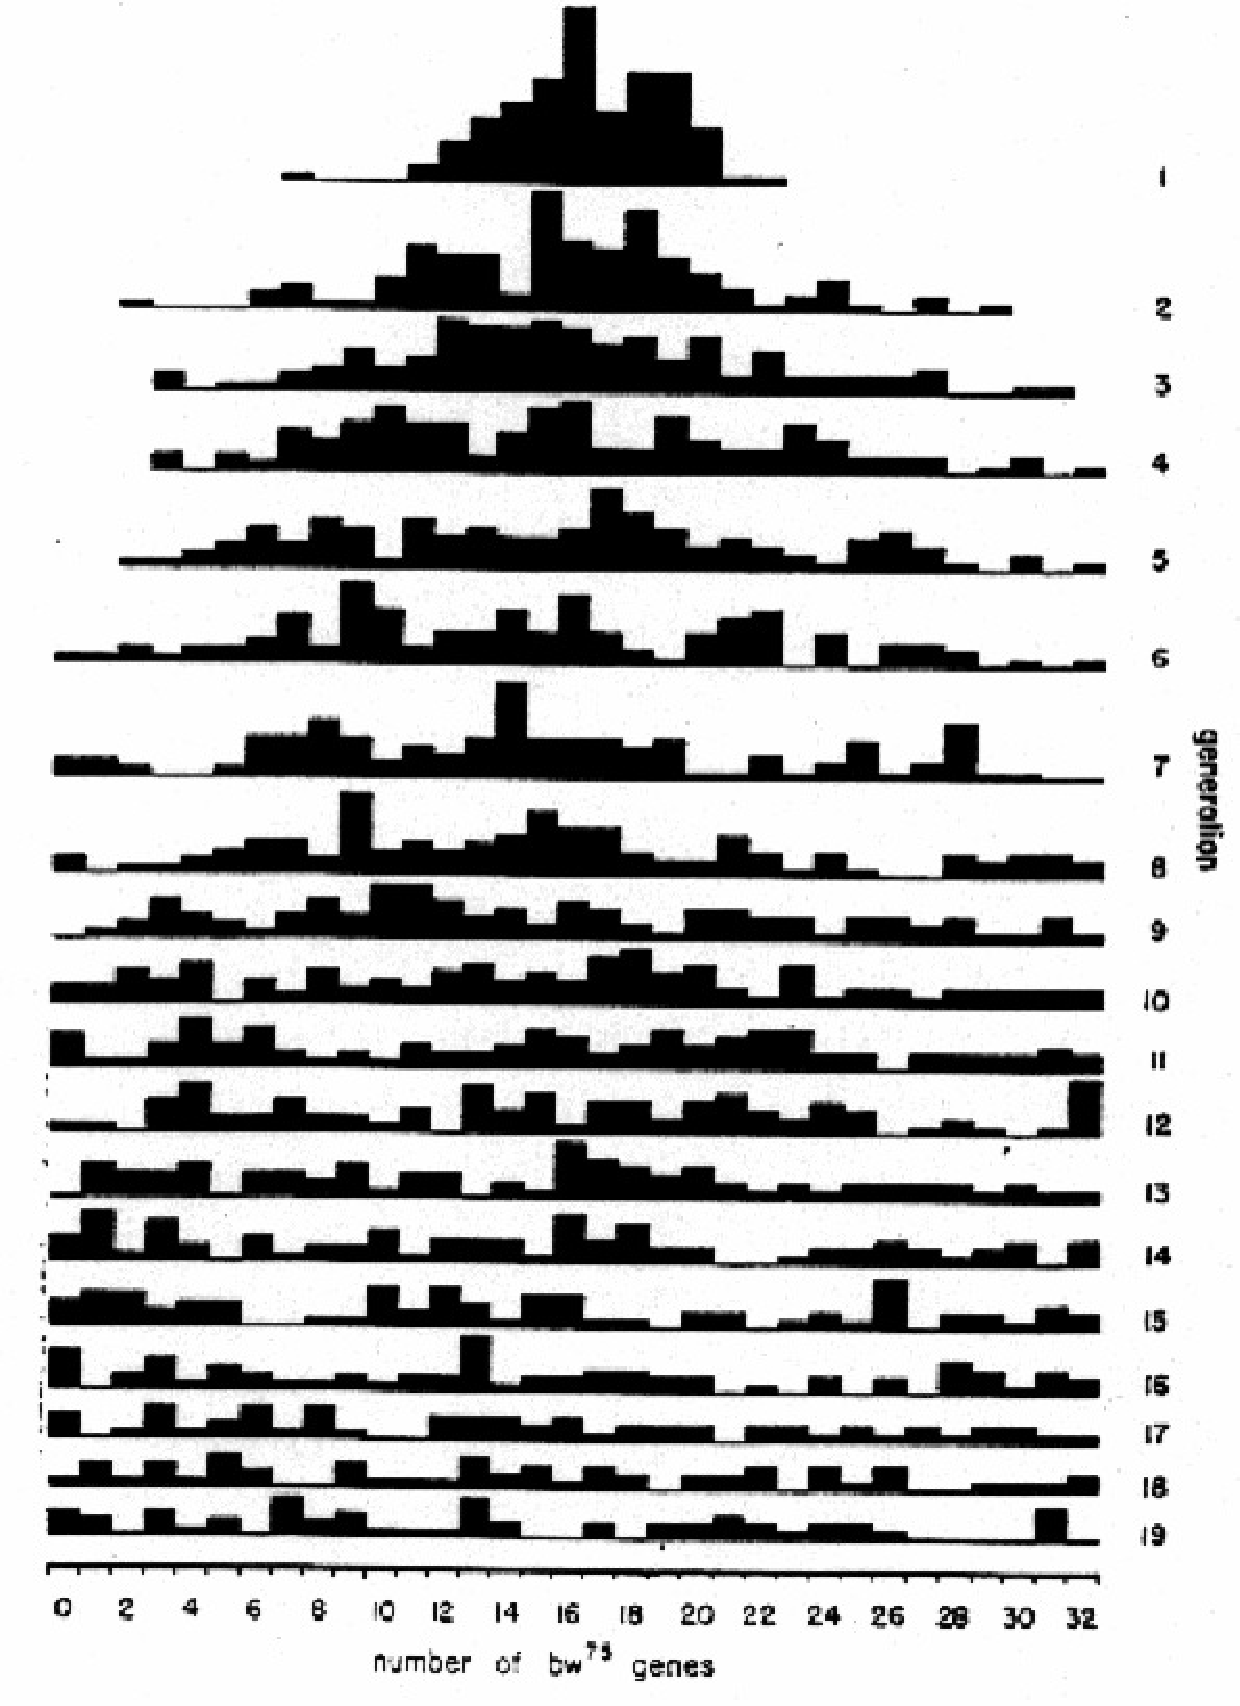
\includegraphics[width=\textwidth]{buridist1.pdf}
\column{0.5\textwidth}
{\bf Buri's drift experiment~I}
\begin{itemize}
\item Each generation: 107 bottles, each w/ 
  8~male \& 8~female fruit flies. 
\item Generation~0: all flies heterozygous.
\item Rows show distribution of allele frequency in 19 successive
  generations. 
\end{itemize}
\mbox{}\hfill \small Peter Buri, 1956
\end{columns}
\end{frame}

%\begin{frame}
%\begin{columns}
%\column{0.6\textwidth}
%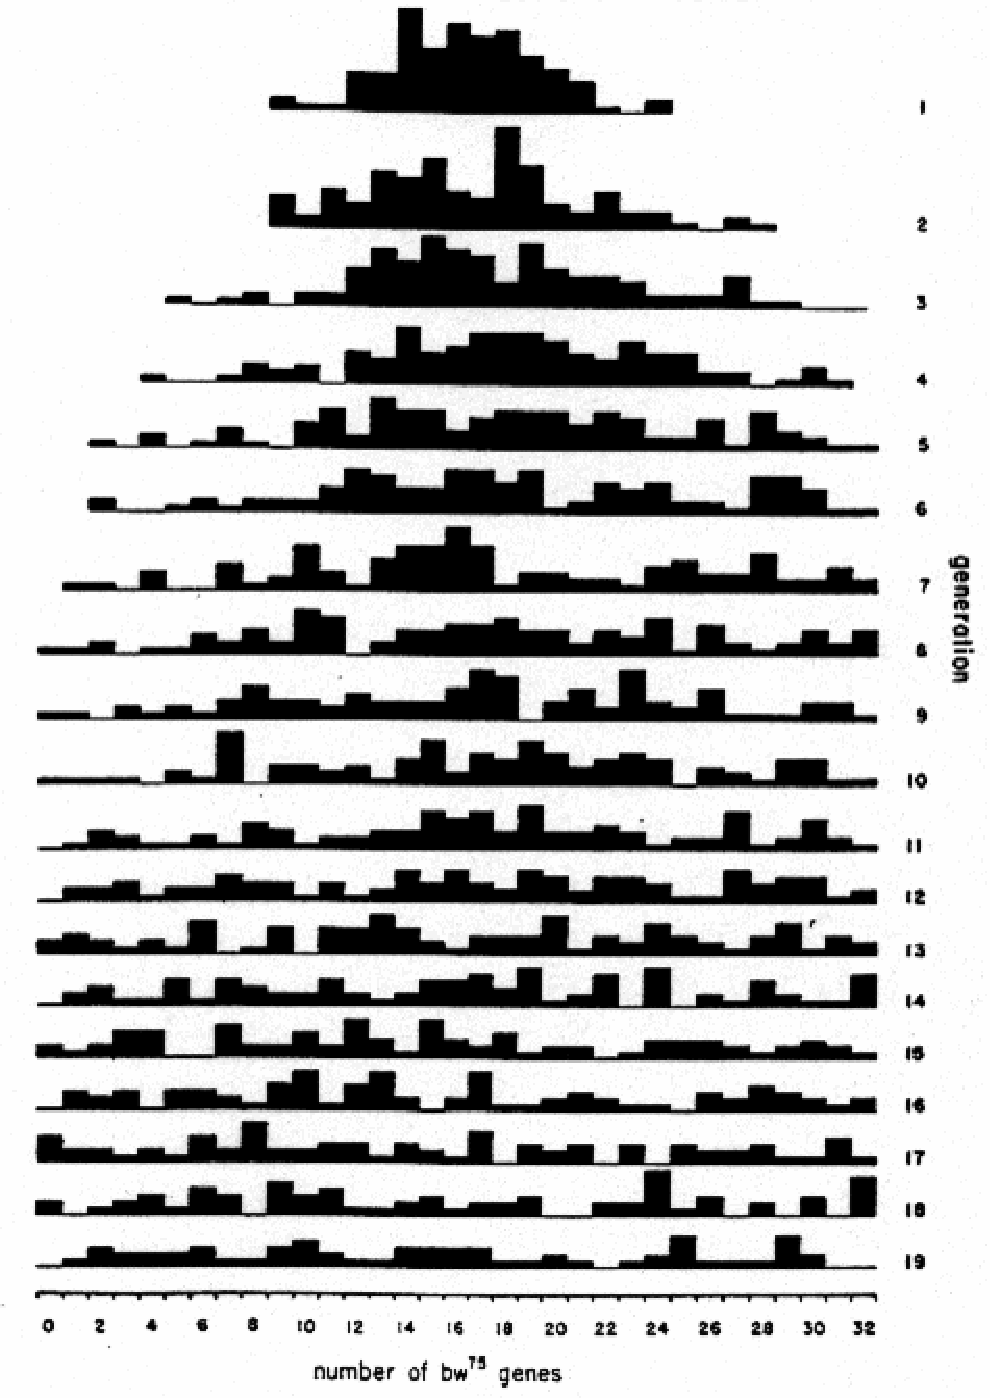
\includegraphics[width=\textwidth]{buridist2.pdf}
%\column{0.5\textwidth}
%{\bf Buri's drift experiment~II}
%\begin{itemize}
%\item Each generation: 105 somewhat larger bottles
%\item Otherwise like experiment~I.
%\end{itemize}
%\mbox{}\hfill \small Peter Buri, 1956
%\end{columns}
%\end{frame}

\begin{frame}
\frametitle{Decay of heterozygosity in Buri's two experiments}
\begin{columns}
\column{0.6\textwidth}
% Buri, Peter. 1956. Gene frequency in small populations
% of mutant drosophila
% Heterozygosity in lines I and II.
\beginpicture
%\setcoordinatesystem units <0.15in, 0.04in>
\setcoordinatesystem units <0.04\textwidth, 0.04in>
\setplotarea x from 1 to 19, y from 0 to 50
\axis left label {$H$}
  ticks withvalues 0.00 0.25 0.50 / at 0 25 50 / /
\axis bottom 
  label {Generation} ticks
  withvalues 1 5 10 15 19 / at 1 5 10 15 19 / /
\put {\footnotesize\begin{tabular}{cl}
  $\bullet$ & Experiment~I\\
  $\circ$   & Experiment~II
  \end{tabular}} [bl] <4pt,4pt> at 1 0
% Heterozygosity in line I
\multiput {$\bullet$} at
%t    H
 1  51.4
 2  46.4
 3  50.4
 4  45.6
 5  44.8
 6  42.8
 7  40.3
 8  40.2
 9  35.8
10  34.8
11  32.5
12  30.5
13  26.3
14  25.5
15  21.6
16  20.2
17  21.0
18  19.7
19  18.3
/
\plot
%t    H
 1  51.4
 2  46.4
 3  50.4
 4  45.6
 5  44.8
 6  42.8
 7  40.3
 8  40.2
 9  35.8
10  34.8
11  32.5
12  30.5
13  26.3
14  25.5
15  21.6
16  20.2
17  21.0
18  19.7
19  18.3
/
% Heterozygosity in line II
\multiput{$\circ$} at
%t    H
 1 49.2
 2 52.9
 3 48.5
 4 45.1
 5 42.7
 6 42.6
 7 40.8
 8 38.0
 9 39.1
10 38.6
11 34.6
12 33.1
13 32.5
14 31.3
15 28.0
16 27.5
17 24.3
18 24.9
19 21.0
/
\plot
%t    H
 1 49.2
 2 52.9
 3 48.5
 4 45.1
 5 42.7
 6 42.6
 7 40.8
 8 38.0
 9 39.1
10 38.6
11 34.6
12 33.1
13 32.5
14 31.3
15 28.0
16 27.5
17 24.3
18 24.9
19 21.0
/
\endpicture
\column{0.4\textwidth}
\begin{itemize}
\item Heterozygosity $(H)$ starts at 0.5
\item Declines to about 0.2
\item Why?
\end{itemize}
\end{columns}
\end{frame}

\begin{frame}
\frametitle{As heterozygosity declined w/i bottles, the variance among
  them increased}
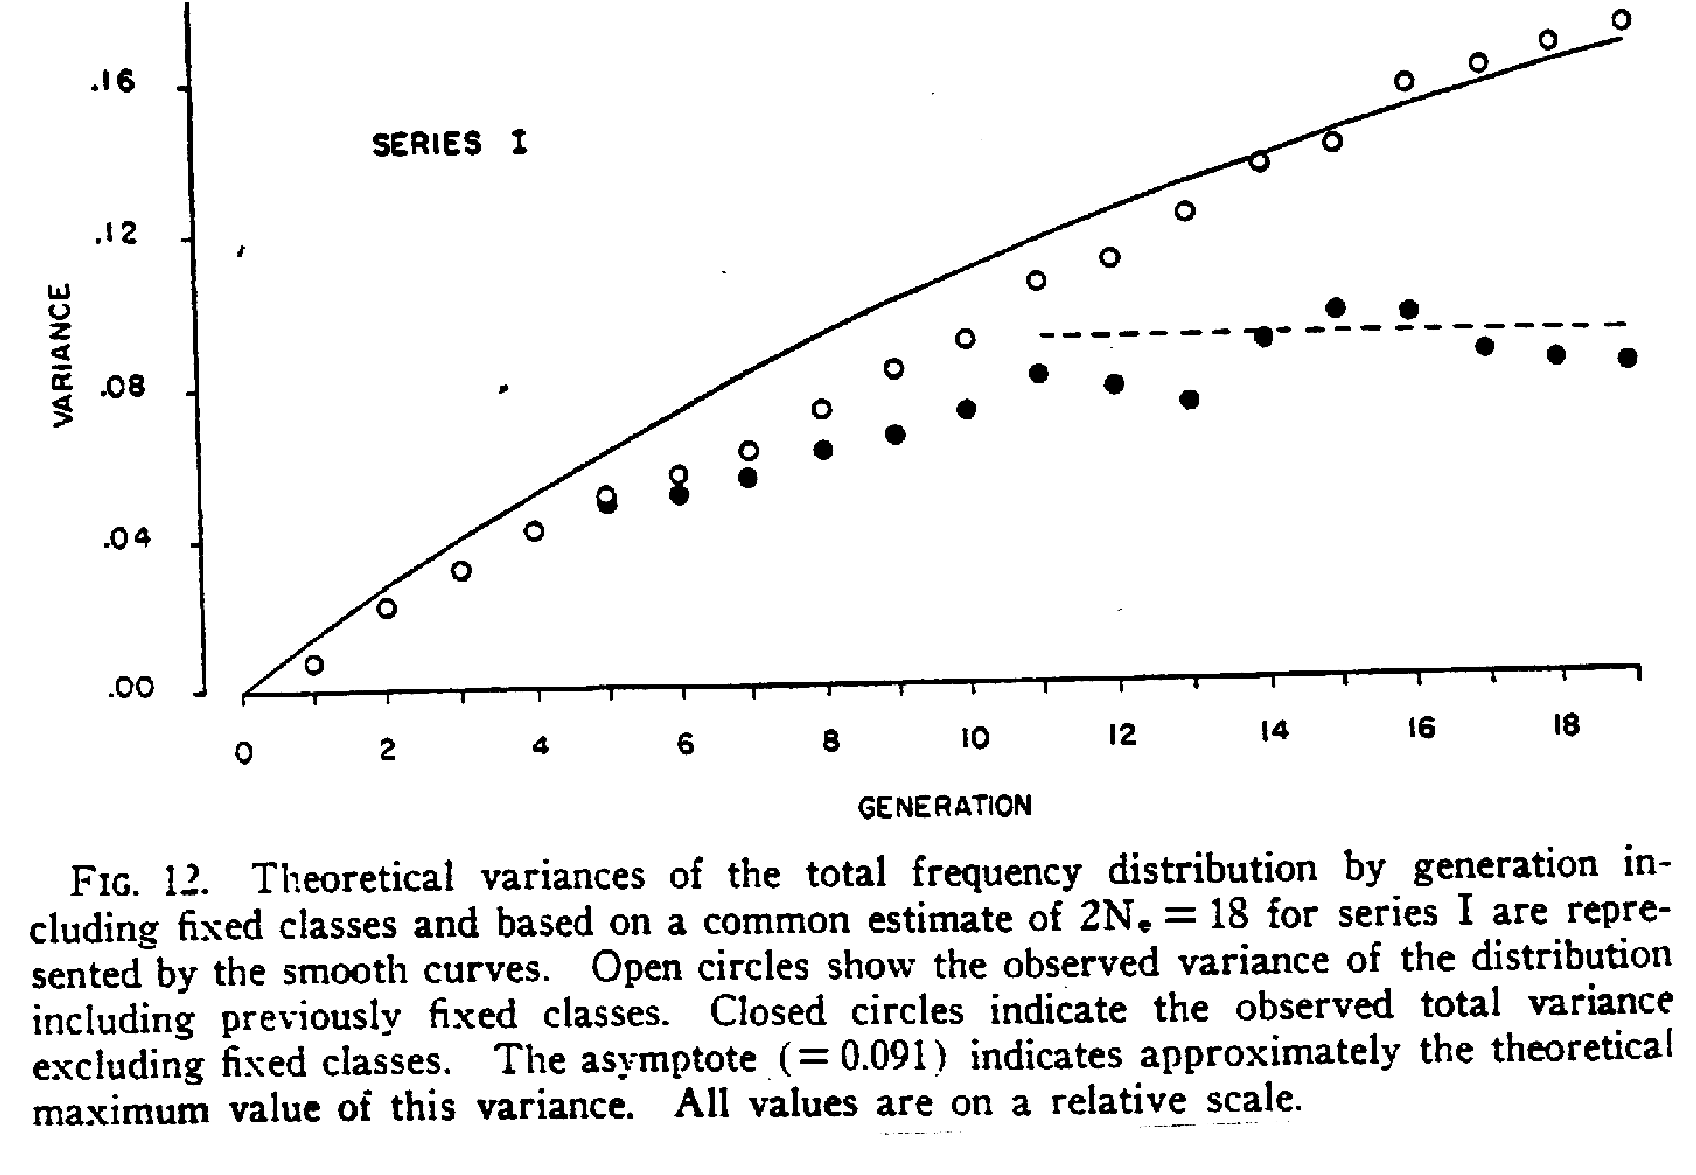
\includegraphics[width=\textwidth]{burivar1.pdf}
\end{frame}

%\begin{frame}
%\frametitle{As heterozygosity declined w/i bottles, the variance among
%  them increased}
%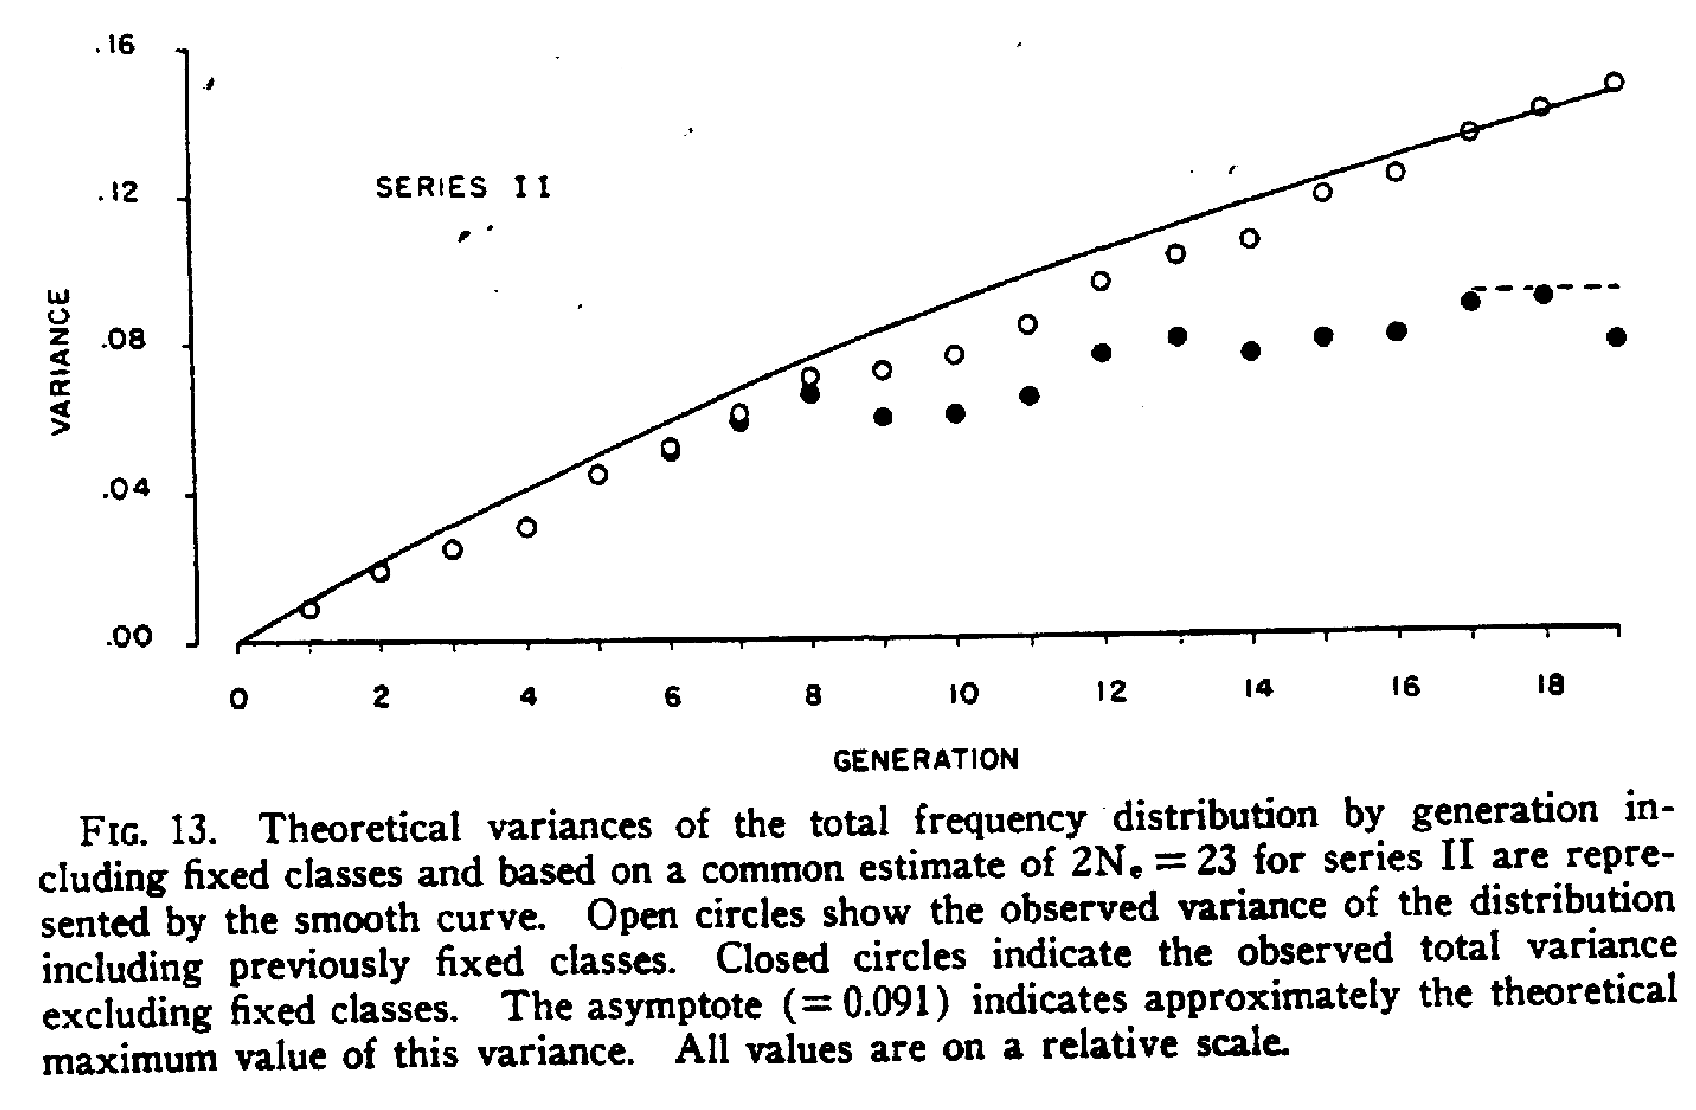
\includegraphics[width=\textwidth]{burivar2.pdf}
%\end{frame}

\begin{frame}
\frametitle{Computer Simulations of Genetic Drift}
\centering
  \mbox{%
  \beginpicture \setcoordinatesystem units <0.016\textwidth,2in> 
  \setplotarea x from 0 to 56, y from 0 to 1
  \axis bottom label {Generations}
  ticks numbered from 0 to 50 by 10 /
  \axis left label {$p$}
  ticks numbered  from 0 to 1 by 0.5 /
  \axis top /
  \axis right /
  \plot 25 0.25 30 0.25 /
  \put  {$2N = 100$} [l] at 31 0.25
% Drift in a population of size 100
\plot
1       0.5000 2        0.4800 3        0.4600 4        0.5200
5       0.4900 6        0.4800 7        0.5100 8        0.5000
9       0.5600 10       0.5900 11       0.6100 12       0.5900
13      0.5500 14       0.5300 15       0.5700 16       0.6200
17      0.6000 18       0.6600 19       0.7200 20       0.7200
21      0.7500 22       0.7100 23       0.6800 24       0.6600
25      0.6100 26       0.5900 27       0.6100 28       0.6000
29      0.7400 30       0.7500 31       0.7300 32       0.7000
33      0.7600 34       0.8300 35       0.9100 36       0.9100
37      0.9000 38       0.9200 39       0.8800 40       0.9200
41      0.9100 42       0.8900 43       0.9000 44       0.8800
45      0.9300 46       0.9500 47       0.9300 48       0.9400
49      0.9500 50       0.9300 51       0.9200 52       0.9200
53      0.9100 54       0.9400 55       0.9100 56       0.9400
/
\setdashes
  \plot 25 0.13 30 0.13 /
  \put {$2N = 20$} [l] at 31 0.13
%N=20
\plot
1 0.5000 2 0.4000 3 0.4500 4 0.4000 5 0.4500 6 0.6500 7 0.6500 8
0.6500 9 0.5500 10 0.6500 11 0.5500 12 0.5000 13 0.5000 14 0.5000 15
0.2500 16 0.1500 17 0.1000 18 0.0500
/
\endpicture}

\end{frame}

\begin{frame}
\frametitle{The Urn Metaphor}

Imagine two urns: metaphors for a population in two successive
generations.  Urn~1 has 50 balls, some red, some white, representing
parental gene copies.  Urn~2 is empty until urn~1 has ``reproduced''
as follows:

\begin{enumerate}
\item Examine a random ball from urn~1.
\item Put a ball of the same color into urn~2.
\item Replace the ball from urn~1.
\item Repeat until there are 50 balls in urn~2.
\end{enumerate}
Urn~2 is differs from urn~1 because of random sampling: a metaphor for
genetic drift.
\end{frame}

\begin{frame}
The urn model behaves a lot like genetic drift in real populations:
\begin{enumerate}
\item variation between populations increases
\item variation within populations decreases
\end{enumerate}
Yet real organisms don't reproduce as our urns do.  The best urn model is
unlikely to be one in which the number of balls matches the number of
gene copies.
\end{frame}

\begin{frame}
\frametitle{Decay of Heterozygosity: Notation}
\begin{tabular}{r@{$\;=\;$}p{4in}}
$N$&\# of diploid individuals in population\\
$2N$&\# of gene copies in population\\
$\G$&Probability that two random gene copies, drawn with
  replacement from generation $t$, are copies of the same allele.\\
$\G'$&same thing in the generation $t+1$.
\end{tabular}
\end{frame}

\begin{frame}
\frametitle{Decay of Heterozygosity: Logic}
Two gene copies may be identical in state either because
\begin{enumerate}
\item they are copies of the same parental gene copy, or 
\item they are copies of distinct parental gene copies, which happen
  to be identical in state. 
\end{enumerate}
\end{frame}

\begin{frame}
\frametitle{Two gene copies either are or are not copies of the same
  parental gene copy} 
\begin{center}
\setlength{\unitlength}{1cm}
\begin{picture}(9,4.6)(-3,-1)
%\put(0,75){\small Generation $t$}
%\put(0,25){\small Generation $t+1$}
\put(0,0){\circle*{2}}
\put(2,0){\circle*{2}}
\put(3.5,0){\circle*{2}}
\put(5.5,0){\circle*{2}}
%
\put(1,3){\circle*{2}}
\put(3.5,3){\circle*{2}}
\put(5.5,3){\circle*{2}}
%
\put(1,3){\vector(-1,-3){0.9}}
\put(1,3){\vector(1,-3){0.9}}
\put(3.5,3){\vector(0,-3){2.7}}
\put(5.5,3){\vector(0,-3){2.7}}
%
\put(-3,2.85){\large Generation 0}
\put(-3,-0.15){\large Generation 1}
\put(0.75,-1){\Large $\frac{1}{2N}$}
\put(4.0,-1){\Large $1-\frac{1}{2N}$}
\end{picture}
\end{center}
Two genes are copies of the same parental gene with probability $1/2N$, and
of distinct parental genes with probability $1-1/2N$.
\end{frame}

\begin{frame}
\begin{center}
\begin{tabular}{|p{3in}|l|}
\hline
Event & Prob\\
\hline
Individual carries 2 copies of same parental gene & $1/2N$\\
\hline
\end{tabular}
\end{center}
Explanation:
\begin{enumerate}
\item First draw a random gamete from among those produced by the parental
  generation.  This gamete is equally likely to have been produced by any of
  the $2N$ parental genes.
\pause
\item Next draw another gamete at random.  There is 1 chance in $2N$
  that the second is a copy of the same parental gene as the first.
\end{enumerate}
\end{frame}

\begin{frame}
\begin{center}
\begin{tabular}{|p{3in}|l|}
\hline
Event & Prob\\
\hline
Individual carries copies of 2 distinct parental genes, which are themselves
  identical. & $(1 - 1/2N)\G$\\
\hline
\end{tabular}
\end{center}
Explanation:
\begin{enumerate}
\item
The two random gene are copies of distinct parental genes with probability
$1 - 1/2N$.
\item
These distinct parental genes are copies of the same allele with probability
$\G$---that is the definition of $\G$.
\item \emph{Both} things are true with probability:
\[\left(1 - \frac{1}{2N}\right) \G\]
\end{enumerate}
\end{frame}

\begin{frame}
In short, the two genes are identical if they are copies either of
\begin{enumerate}
\item the same parental gene (probability $1/2N$), or of
\item distinct but identical genes (probability $(1 - 1/2N)\G$).
\end{enumerate}
Altogether,
\[
\G' = \frac{1}{2N} + \left(1 - \frac{1}{2N}\right) \G
\]
\end{frame}

\begin{frame}
To see where this goes, it is easier to work with the probability that the two
genes are copies of \emph{different} alleles, i.e.\ with the heterozygosity,
\begin{eqnarray*}
\Het' &=& 1-\G'\\
%&=& 1 - \frac{1}{2N} - \left(1 - \frac{1}{2N}\right) \G\\
%&=& \left(1 - \frac{1}{2N}\right)(1-\G)\\
&=& \left(1 - \frac{1}{2N}\right)\Het \qquad \mbox{(after some algebra).}\\
\end{eqnarray*}
Can you supply the algebra?
\end{frame}

\begin{frame}
\frametitle{The Time-path of Heterozygosity}
\begin{eqnarray*}
\Het_1 &=& \left(1 - \frac{1}{2N}\right)\Het_0\\[4pt]
\pause
\Het_2 &=& \left(1 - \frac{1}{2N}\right)\Het_1\\[4pt]
\pause
       &=& \left(1 - \frac{1}{2N}\right)^2\Het_0\\[4pt]
\pause
\Het_t &=& \left(1 - \frac{1}{2N}\right)^t\Het_0\\
\end{eqnarray*}
where $\Het_0$ is the original heterozygosity and $\Het_t$ is the
heterozygosity in generation $t$.
\end{frame}

\begin{frame}
\frametitle{Example}
In Peter Buri's experiment, $\Het_1=1/2$ because half the population were
heterozygotes after the first generation of random mating.

18 generations later:
\[
\Het_{19} = \frac{1}{2} \left(1 - \frac{1}{2N}\right)^{18}
\]

But what is $2N$?
\end{frame}

\begin{frame}
\frametitle{Heterozygosity: Buri's experiment~I vs.\ urn model}
% Buri, Peter. 1956. Gene frequency in small populations
% of mutant drosophila
% Heterozygosity in lines I and II.
\beginpicture
%\setcoordinatesystem units <0.15in, 0.04in>
\setcoordinatesystem units <0.035\textwidth, 0.04in>
\setplotarea x from 1 to 19, y from 0 to 50
\axis left label {$H$}
  ticks withvalues 0.00 0.25 0.50 / at 0 25 50 / /
\axis bottom 
  label {Generation} ticks
  withvalues 1 5 10 15 19 / at 1 5 10 15 19 / /
% Heterozygosity in line I
\multiput {$\bullet$} at
%t    H
 1  51.4
 2  46.4
 3  50.4
 4  45.6
 5  44.8
 6  42.8
 7  40.3
 8  40.2
 9  35.8
10  34.8
11  32.5
12  30.5
13  26.3
14  25.5
15  21.6
16  20.2
17  21.0
18  19.7
19  18.3
/
\setbox0=\hbox{$2N=18$}%
\put {$2N=18$\raise\ht0\hbox{$\nearrow$}} [tr] at 9   31.7
%2N = 18
\plot   
 1   50.0
 2   47.2
 3   44.6
 4   42.1
 5   39.8
 6   37.6
 7   35.5
 8   33.5
 9   31.7
10   29.9
11   28.2
12   26.7
13   25.2
14   23.8
15   22.5
16   21.2
17   20.0
18   18.9
19   17.9
/
\setbox0=\hbox{$\swarrow$}%
\put {$\swarrow$\raise\ht0\hbox{$2N=32$}} [bl] at 15 32.1
%2N=32
\plot
1 50.0
 2 48.4
 3 46.9
 4 45.5
 5 44.0
 6 42.7
 7 41.3
 8 40.0
 9 38.8
10 37.6
11 36.4
12 35.3
13 34.2
14 33.1
15 32.1
16 31.1
17 30.1
18 29.1
19 28.2
/
\endpicture 

\end{frame}

\begin{frame}
\frametitle{Heterozygosity: Buri's experiment~I vs.\ urn model}
\begin{columns}
\column{0.5\textwidth}
% Buri, Peter. 1956. Gene frequency in small populations
% of mutant drosophila
% Heterozygosity in lines I and II.
\beginpicture
%\setcoordinatesystem units <0.15in, 0.04in>
\setcoordinatesystem units <0.035\textwidth, 0.04in>
\setplotarea x from 1 to 19, y from 0 to 50
\axis left label {$H$}
  ticks withvalues 0.00 0.25 0.50 / at 0 25 50 / /
\axis bottom 
  label {Generation} ticks
  withvalues 1 5 10 15 19 / at 1 5 10 15 19 / /
% Heterozygosity in line I
\multiput {$\bullet$} at
%t    H
 1  51.4
 2  46.4
 3  50.4
 4  45.6
 5  44.8
 6  42.8
 7  40.3
 8  40.2
 9  35.8
10  34.8
11  32.5
12  30.5
13  26.3
14  25.5
15  21.6
16  20.2
17  21.0
18  19.7
19  18.3
/
\setbox0=\hbox{$2N=18$}%
\put {$2N=18$\raise\ht0\hbox{$\nearrow$}} [tr] at 9   31.7
%2N = 18
\plot   
 1   50.0
 2   47.2
 3   44.6
 4   42.1
 5   39.8
 6   37.6
 7   35.5
 8   33.5
 9   31.7
10   29.9
11   28.2
12   26.7
13   25.2
14   23.8
15   22.5
16   21.2
17   20.0
18   18.9
19   17.9
/
\setbox0=\hbox{$\swarrow$}%
\put {$\swarrow$\raise\ht0\hbox{$2N=32$}} [bl] at 15 32.1
%2N=32
\plot
1 50.0
 2 48.4
 3 46.9
 4 45.5
 5 44.0
 6 42.7
 7 41.3
 8 40.0
 9 38.8
10 37.6
11 36.4
12 35.3
13 34.2
14 33.1
15 32.1
16 31.1
17 30.1
18 29.1
19 28.2
/
\endpicture 

\column{0.5\textwidth}
\begin{itemize}
\item There were 32 gene copies in each bottle.
\item Yet $2N=32$ provides a poor fit to data.
\item Better fit with $2N=18$.
\item 18 is the ``\emph{effective population size}''
\end{itemize}
\end{columns}
\end{frame}

\begin{frame}
\frametitle{$F_{ST}$ measures variation among populations}
\begin{center}
\mbox{%
\sf
\beginpicture
%%%%%%%%%%%%%% left plot
\setcoordinatesystem units <0.075in, 7.35in> point at 19 0
\setplotarea x from 0 to 19, y from 0 to 0.17
\axis left label {$F_{st}$}
  ticks numbered from 0.0 to 0.15 by  0.05 /
\axis bottom   label {Generation} 
  ticks numbered from 0 to 15 by 5 /
\plotheading{Data from Buri (1956)}
\put {Series I} [rb] at 19 0.01
%data
\multiput {$\bullet$} at
%Gen.      FstI
   0  0.0000000
   1  0.0060000
   2  0.0260000
   3  0.0310000
   4  0.0420000
   5  0.0500000
   6  0.0550000
   7  0.0620000
   8  0.0720000
   9  0.0830000
  10  0.0900000
  11  0.1050000
  12  0.1120000
  13  0.1230000
  14  0.1360000
  15  0.1400000
  16  0.1550000
  17  0.1600000
  18  0.1650000
  19  0.1700000
/
%%%%%%%%%%%%%% right plot
\setcoordinatesystem units <0.075in, 7.35in> point at -1 0
\setplotarea x from 0 to 19, y from 0 to 0.17
\axis right label {$F_{st}$}
  ticks numbered from 0.0 to 0.15 by  0.05 /
\axis bottom   label {Generation} 
  ticks numbered from 0 to 15 by 5 /
\put {Series II} [rb] at 19 0.01
%data
\multiput {$\bullet$} at
%Gen.     FstII
   0  0.0000000
   1  0.0090000
   2  0.0180000
   3  0.0240000
   4  0.0300000
   5  0.0450000
   6  0.0520000
   7  0.0600000
   8  0.0700000
   9  0.0720000
  10  0.0760000
  11  0.0840000
  12  0.0940000
  13  0.1010000
  14  0.1050000
  15  0.1170000
  16  0.1220000
  17  0.1330000
  18  0.1390000
  19  0.1440000
/
\endpicture}
\end{center}


%%% Local Variables: 
%%% mode: latex
%%% TeX-master: t
%%% End: 

\end{frame}

\begin{frame}
\frametitle{Model fits after setting $N=N_e$}
\begin{center}
\mbox{%
\sf
\beginpicture
%%%%%%%%%%%%%% left plot
\setcoordinatesystem units <0.075in, 7.35in> point at 19 0
%\setcoordinatesystem units <0.151in, 14.7in> point at 19 0
\setplotarea x from 0 to 19, y from 0 to 0.17
\axis left label {$F_{st}$}
  ticks numbered from 0.0 to 0.15 by  0.05 /
\axis bottom   label {Generation} 
  ticks numbered from 0 to 15 by 5 /
\plotheading{Data from Buri (1956)}
\put {Series I} [rb] at 19 0.04
\put {\small $2N_e=18$} [rb] at 19 0.01
\put {\begin{tabular}{cl}
$\circ$ & theory\\
$\bullet$ & data
\end{tabular}} [lt] at 1 0.17
\multiput {$\circ$} at
%Gen.     EFstI
   0  0.0000000
   1  0.0138889
   2  0.0270062
   3  0.0393947
   4  0.0510950
   5  0.0621453
   6  0.0725817
   7  0.0824382
   8  0.0917472
   9  0.1005390
  10  0.1088424
  11  0.1166845
  12  0.1240909
  13  0.1310859
  14  0.1376922
  15  0.1439315
  16  0.1498242
  17  0.1553896
  18  0.1606457
  19  0.1656098
/
\multiput {$\bullet$} at
%Gen.      FstI
   0  0.0000000
   1  0.0060000
   2  0.0260000
   3  0.0310000
   4  0.0420000
   5  0.0500000
   6  0.0550000
   7  0.0620000
   8  0.0720000
   9  0.0830000
  10  0.0900000
  11  0.1050000
  12  0.1120000
  13  0.1230000
  14  0.1360000
  15  0.1400000
  16  0.1550000
  17  0.1600000
  18  0.1650000
  19  0.1700000
/
%%%%%%%%%%%%%% right plot
\setcoordinatesystem units <0.075in, 7.35in> point at -1 0
%\setcoordinatesystem units <0.15in, 14.7in> point at -1 0
\setplotarea x from 0 to 19, y from 0 to 0.17
\axis right label {$F_{st}$}
  ticks numbered from 0.0 to 0.15 by  0.05 /
\axis bottom   label {Generation} 
  ticks numbered from 0 to 15 by 5 /
\put {Series II} [rb] <-0.5ex,0pt> at 19 0.04
\put {\small $2N_e=23$} [rb] <-0.5ex,0pt> at 19 0.01
%theory
\multiput {$\circ$} at
%Gen.  EFstII
   0  0.00000
   1  0.01087
   2  0.02127
   3  0.03121
   4  0.04072
   5  0.04982
   6  0.05853
   7  0.06685
   8  0.07481
   9  0.08243
  10  0.08972
  11  0.09669
  12  0.10335
  13  0.10973
  14  0.11583
  15  0.12166
  16  0.12724
  17  0.13258
  18  0.13768
  19  0.14257
/
\multiput {$\bullet$} at
%Gen.     FstII
   0  0.0000000
   1  0.0090000
   2  0.0180000
   3  0.0240000
   4  0.0300000
   5  0.0450000
   6  0.0520000
   7  0.0600000
   8  0.0700000
   9  0.0720000
  10  0.0760000
  11  0.0840000
  12  0.0940000
  13  0.1010000
  14  0.1050000
  15  0.1170000
  16  0.1220000
  17  0.1330000
  18  0.1390000
  19  0.1440000
/
\endpicture}
\end{center}


%%% Local Variables: 
%%% mode: latex
%%% TeX-master: t
%%% End: 

\end{frame}
